\documentclass[10pt,letterpaper]{article}
\usepackage[margin=0.9in]{geometry}
\usepackage[T1]{fontenc}
\usepackage{lmodern,microtype}
\usepackage{amsmath,amssymb,booktabs,tabularx,array}
\usepackage{enumitem,xcolor,tikz}
\usetikzlibrary{arrows.meta,positioning,fit}
\usepackage{fancyhdr}
\usepackage[colorlinks=true,linkcolor=blue!45!black,citecolor=blue!45!black,urlcolor=blue!45!black]{hyperref}
\usepackage{url}
\hypersetup{pdftitle={Generalist: An Interactive Agent Runtime with Executable Protocol Models},
pdfauthor={Generalist Project},pdfsubject={Architecture and bounded verification},
pdfkeywords={agent runtime, TLA+, trace validation, Rust}}
\definecolor{ink}{HTML}{163047}
\definecolor{accent}{HTML}{226A72}
\definecolor{pale}{HTML}{EEF4F5}
\setlength{\parindent}{0pt}
\setlength{\parskip}{5pt plus 1pt}
\setlength{\emergencystretch}{2em}
\setlist{nosep,leftmargin=1.5em}
\pagestyle{fancy}
\fancyhf{}
\fancyhead[L]{\small\textcolor{ink}{GENERALIST}}
\fancyhead[R]{\small Technical whitepaper / September 2026}
\fancyfoot[C]{\small\thepage}
\setlength{\headheight}{14pt}
\newcommand{\tla}{TLA\textsuperscript{+}}
\newcommand{\code}[1]{\texttt{#1}}
\newcolumntype{Y}{>{\raggedright\arraybackslash}X}
\title{\vspace{-1.5em}\textcolor{ink}{\Huge Generalist}\\[0.6em]
\Large An Interactive Agent Runtime with\\Executable Protocol Models}
\author{Generalist Project}
\date{September 2026}

\begin{document}
\maketitle
\thispagestyle{fancy}
\begin{abstract}
Generalist is a Unix command-line agent implemented in Rust. It combines a
provider-independent conversation loop, an interactive terminal controller,
permissioned tools, Python orchestration, and explicit project-scoped archives.
The design problem examined here is how to preserve user intent and valid
conversation state while provider requests, tool execution, cancellation,
permissions, and persistence proceed asynchronously.

Three finite \tla{} specifications describe conversation ownership, episodic
capture, and archive scope routing. A deterministic harness records selected
implementation actions and checks them against the original specification
operators. Deliberate trace corruptions and model faults test whether the gate
rejects meaningful violations. Expanding the harness exposed four gaps in the
previous specification/instrumentation connection; a separate Rust regression
exposed steering consumption after cancellation at a truncated-response
boundary. This paper explains the implementation, the corrections, and the
scope of the evidence. The result is bounded model checking and sampled
implementation validation, with explicit assumptions about event observation,
external effects, and durability.
\end{abstract}

\section{Problem and design priorities}
An agent's control loop is short in outline: send history to a model, execute
requested tools, append results, and request another completion. The surrounding
runtime is harder. A user can submit another instruction while a request is
pending, deny a tool, edit a queue, or interrupt work while an external process
is changing files. An autosave may lag behind accepted input. A provider can
return a partial tool call, duplicate call identifiers, an unexpected native
tool name, or an error after earlier tools have already run.

Generalist treats these as protocol problems with identifiable owners and
transition boundaries. It aims to preserve stable prompt identity, paired tool
history, correlated permission decisions, and explicit archive scope. It also
keeps the terminal responsive without making rendered text the authority for
conversation state. These properties are useful even when the language model's
reasoning or final answer is wrong.

The contribution of this artifact is an implementation and an auditable
verification workflow. It is not a new language-model training method or a
claim of priority for agent orchestration or trace validation. ReAct studies
interleaved reasoning and actions; SWE-agent studies interfaces through which
models operate on software environments \cite{yao2023react,yang2024sweagent}.
Generalist's focus here is the host protocol around such interactions. This
paper reports no comparative task-success or inference-speed result.

\section{Architecture and authority}
The library separates the agent loop from provider adapters, tools, and the
terminal interface. \path{src/agent/} owns conversation mutation. The binary
controller in \path{src/main.rs} and \path{src/tui/} coordinates terminal input,
permission events, queue changes, and display updates. \path{src/runtime.rs}
contains shared queue claims and cancellation controls. Provider adapters use
one completion vocabulary; local inference is an optional feature.

\begin{figure}[ht]
\centering
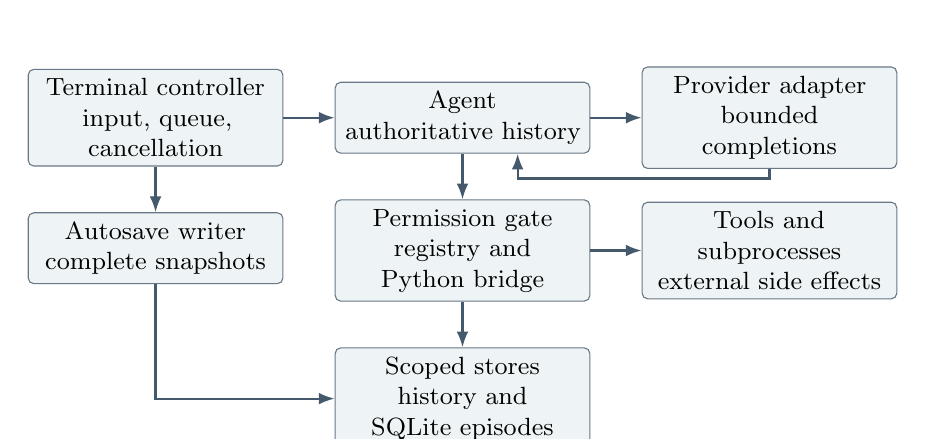
\begin{tikzpicture}[
  node distance=0.58cm and 0.65cm,
  box/.style={draw=ink!65,rounded corners=2pt,fill=pale,align=center,
    text width=3.0cm,minimum height=0.9cm,font=\small},
  arr/.style={-{Latex[length=2mm]},draw=ink!80,thick}]
\node[box] (ui) {Terminal controller\\input, queue, cancellation};
\node[box,right=of ui] (agent) {Agent\\authoritative history};
\node[box,right=of agent] (provider) {Provider adapter\\bounded completions};
\node[box,below=of agent] (gate) {Permission gate\\registry and Python bridge};
\node[box,right=of gate] (tools) {Tools and subprocesses\\external side effects};
\node[box,below=of ui] (save) {Autosave writer\\complete snapshots};
\node[box,below=of gate] (archive) {Scoped stores\\history and SQLite episodes};
\draw[arr] (ui) -- (agent);
\draw[arr] (agent) -- (provider);
\draw[arr] (provider.south) -- ++(0,-0.12) -| ([xshift=0.7cm]agent.south);
\draw[arr] (agent) -- (gate);
\draw[arr] (gate) -- (tools);
\draw[arr] (ui) -- (save);
\draw[arr] (gate) -- (archive);
\draw[arr] (save) |- (archive);
\end{tikzpicture}
\caption{Ownership and principal data paths. Display events are projections;
external tool effects are not rolled back by conversation cancellation.}
\label{fig:architecture}
\end{figure}

One Tokio task polls the terminal reactor and the non-\code{Send} agent future.
The prompt queue uses \code{Rc<RefCell<...>>}; this expresses single-thread
ownership rather than a cross-thread scheduling protocol. Blocking persistence
work is delegated to dedicated workers. The model describes abstract control
locations, while the implementation uses Rust ownership, structured control
flow, and RAII claims. It does not maintain a second mutable copy of every
model variable.

\begin{table}[ht]
\small
\begin{tabularx}{\linewidth}{@{}p{0.25\linewidth}YY@{}}
\toprule
State & Authoritative owner & Derived or delayed view \\
\midrule
Conversation and active goal & Agent, then controller at a valid checkpoint & Terminal transcript and autosave snapshot \\
Queued input & Shared prompt queue with stable IDs & Queue modal and restored composer text \\
Permission request & Permission handler/broker for a live invocation & Modal or remembered-policy notification \\
Saved conversation & Scope-bound history store & Sanitized archive search result \\
Episode capture & One SQLite worker per opened memory client & Status, search summaries, and exported text \\
\bottomrule
\end{tabularx}
\caption{Authority is separate from presentation and asynchronous persistence.}
\end{table}

\subsection{Prompt identity, delivery, and settlement}
Every queued prompt has an ID, text, delivery mode, and origin. Equal text does
not imply equal identity. A follow-up begins another turn; a steer is eligible
for the active turn's next valid history boundary. With no active turn, the
controller admits follow-ups. After settlement, residual steers become
follow-ups because their previous owner no longer exists.

A two-phase claim removes entries from the visible queue. Committing a claim
records their delivery; dropping an uncommitted claim restores them to the
front. The controller records the initial user message and commits its start
claim without an intervening await. Steering similarly claims all eligible
entries in relative FIFO order, appends them to valid history, and commits the
claim synchronously. Queue edits address IDs, so duplicate text and concurrent
presentation changes do not select another item accidentally.

An optional persistent goal is host instruction state. Normal turn settlement
can schedule one host-authored follow-up while the objective remains active.
The reserved \code{update\_goal} control is owned by the agent and cannot be
registered or shadowed as an ordinary capability. Host continuation provenance
survives queueing and persistence and is omitted from episodic user text.
The implementation's completion control records the model's completion signal;
it does not independently prove that the user's real-world objective was met.

\subsection{History is the transaction boundary}
An accepted assistant tool-use batch must receive exactly one result per call
in the immediately following user message. The executable predicate
\code{history\_tool\_protocol\_is\_valid} checks matching IDs, duplicates,
orphan results, and role placement. Invalid protocol boundaries cannot be
persisted through the history store. The agent retains earlier valid history
when a later provider request fails.

A provider response is accepted only after host byte, block, and tool-count
limits pass. Streamed text is a preview until the full response is committed.
Refusal and truncated tool calls produce synthetic results instead of executing
the affected calls. A normal tool denial stops later calls in the same outer
batch and pairs each skipped call. Cooperative cancellation pairs unfinished
calls with an explicit unknown-completion result. This protects the next
provider request's protocol; it cannot undo a file edit or network operation.

At cancellation boundaries, a completed future and an interrupt may both be
ready. Tokio's selection semantics make cancellation safety a property of the
chosen operations and their ownership, not merely of using \code{select!}
\cite{tokioselect}. Generalist rechecks cancellation before consuming steering
after a tool batch. The audit extended that check to the synthetic-result path
for truncated responses.

\section{Tools, permissions, and trust boundaries}
By default, the model-facing capability is a Python runner. It can invoke
registered capabilities through a generated \code{tools} module, allowing
several calls within one provider round. Tool definitions are stable in
registration order, and large code-only schemas can be disclosed on demand.
An undeclared native call is returned as a protocol error without permission
checking or execution. A library caller may disable code mode or supply a
registered Python capability, so this default is not universal to every library
configuration.

The outer script and its bridged calls pass through the registry's shared
permission entry point. Remembered ordinary-tool policy and session-only exact
input grants remain separate. Archive operations receive an additional
structural capability: only the registry can construct a
\code{ToolAuthorization} after approving the exact name and JSON input. An
archive tool derives a narrower \code{DisclosureGrant} binding operation,
filter, query or identifier, and expected returned scope. Public cross-scope
storage APIs recheck that grant. This makes omission of an ordinary permission
call insufficient to obtain a storage capability.

\subsection{Why a denied request is not a completed tool}
The outer tool/result protocol and the permission protocol have different
granularity. Consider one Python call that catches two denied bridge requests:
\begin{center}
\small
\begin{tabular}{@{}ll@{}}
\toprule
Observed action & Outstanding outer results \\
\midrule
\code{ProviderToolBatch(1)} & 1 \\
Allow the Python request & 1 \\
Deny the first bridge request & 1 \\
Deny the second bridge request & 1 \\
\code{CompleteTool} for Python & 0 \\
\code{SettleTurn} & 0 \\
\bottomrule
\end{tabular}
\end{center}
The earlier model incremented its result counter during \code{DenyPermission}.
That conflated an inner decision with an outer result. The corrected action
retires the live request and marks a denial; result accounting is a separate
\code{CompleteTool} transition. Trace emission is shared by registered tools
and the built-in runner, so outer Python decisions no longer disappear from
observed executions. A script may catch bridge errors, but the host still
propagates the denial in the outer structured outcome.

\subsection{Subprocess containment}
The normal CLI configures project-scoped subprocess policies for Python, shell,
patch, and solver execution. The implementation includes macOS Seatbelt and
Linux Landlock/seccomp or Bubblewrap paths. Landlock is an unprivileged kernel
access-control mechanism whose supported rights depend on the available ABI
\cite{landlock}. Generalist must check concrete platform support; a model of
permission requests does not validate a kernel sandbox.

Subprocess ownership includes bounded I/O, timeouts, and process-group cleanup.
There are no aggregate CPU, memory, process, or disk quotas. In particular,
macOS cleanup cannot guarantee finding an adversarial child that changes
process group and is reparented. Host file tools, configured MCP servers,
unrestricted library defaults, and an explicitly selected host bypass mode
have their own authority. The system is a local developer tool with layered
controls, not a hostile multi-tenant isolation boundary. These controls do not
establish prompt-injection resistance or truthfulness of model-generated text.

\section{Persistence and explicit memory}
Project scope is derived from the workspace; global scope is a deliberate
choice. A global archive is not an implicit fallback when the current project
has no results. The scope-bound history store rejects state claiming a
different scope. Cross-scope model reads require categorical filters and the
structural grant described above. Host inspection commands and model-mediated
archive access are distinct entry points.

An autosave checkpoint contains a complete valid history boundary, goal,
remembered policy, and queue. The controller sends it to a dedicated writer
that may coalesce waiting snapshots. File writes use a temporary file, flush,
atomic replacement, and parent-directory flush. A checkpoint event means that
the in-memory boundary is accepted, not that disk already contains it. Orderly
shutdown flushes pending work or reports failure. A process crash before the
new snapshot is written can lose the latest accepted state while retaining the
previous complete save. The \tla{} models do not include this disk queue or
crash recovery.

Episodic memory is an opt-in inspection feature. A worker records a bounded
projection of a settled turn: user and assistant text, provider/model and
outcome metadata, tool names, and result error flags. Retention types cannot
carry tool inputs, tool-result bodies, reasoning, signatures, or redacted
reasoning payloads. This is structural omission of particular channels; user
or assistant prose can still contain secrets. There is no general secret
redactor.

The worker uses SQLite transactions and WAL. SQLite documents atomic commit
and WAL checkpoint behavior separately \cite{sqliteatomic,sqlitewal}; a green
Generalist model cannot substitute for those storage assumptions. Paused
capture skips publication, insertion failure must publish no partial row, and
forgetting removes a current live row. Deletion does not erase prior exports,
backups, or text already disclosed into a conversation. The request channel
and live store have no quota. There is no automatic retrieval into prompts,
model-authored memory-write tool, consolidation service, or collaborative
memory protocol in the implemented prototype.

\section{What the formal models say}
A \tla{} specification describes initial states and allowed transitions;
safety properties constrain reachable states, while temporal properties require
explicit progress assumptions \cite{lamport2002}. Generalist uses three
separate finite specifications. Their constants define the checked instances,
not an unbounded theorem about every queue length or runtime execution.

\begin{table}[ht]
\small
\begin{tabularx}{\linewidth}{@{}p{0.23\linewidth}YY@{}}
\toprule
Model & Principal state and safety & Progress boundary \\
\midrule
\code{AsyncRuntime} & One active turn; unique queue/claim identities; tool-result counts; live permission ownership; committed history order & Busy periods settle under controller fairness, including eventual permission resolution \\
\code{MemoryRuntime} & Immutable current scope; FIFO pending episodes; disjoint live/skipped/failed/forgotten lifecycle; permissioned disclosure & Pending episodes resolve under fairness of processing the queue head \\
\code{ArchiveScopeRuntime} & Explicit startup scope; writes remain in active scope; a representative disclosure matches its request and authorization witness & Safety only; no retrieval or filesystem liveness theorem \\
\bottomrule
\end{tabularx}
\caption{Each specification abstracts different authoritative state. The repository does not prove their composition.}
\label{tab:models}
\end{table}

For the async model, key predicates include
\[
  \text{toolResults}\leq\text{toolUses},\qquad
  \text{phase}=\text{idle}\ \Longleftrightarrow\
  \text{activeTurn}=\text{NoPrompt}.
\]
At a history-valid boundary, tool counts must agree. Queue identities and
committed prompt order are checked separately, because equal counts alone
cannot establish correct pairing or prompt delivery. The Rust history
predicate checks concrete tool IDs; the finite async model abstracts tools to
counts and permission requests to fresh abstract identities.

\subsection{Fairness and finite bounds}
The checked async configuration contains three prompt IDs, two request IDs,
up to two tools per response, two provider rounds, and one recoverable claim
failure. Weak fairness of agent progress assumes that enabled controller
work, including a pending permission decision, eventually proceeds. Finite
prompt, request, round, and failure budgets are part of the termination
argument. Copy-mode rendering is abstracted away: automatic permission
decisions and host goal scheduling may progress while a frame is paused.
The previous display-state guards incorrectly blocked both cases. Removing
that state also removes an eventual-resume property that merely restated its
fairness assumption; terminal behavior remains a concrete test obligation.

The memory configuration has two episode IDs and three scope labels, with a
fixed current project. The archive configuration has three scopes, two history
IDs, and two memory IDs, including representative pre-existing global and
foreign records. The memory model does not itself trace arbitrary pre-existing
foreign database contents. None of these bounds proves that a live provider,
a filesystem, or an external tool eventually returns. Model-checker
fingerprints also have a nonzero collision probability.

\subsection{Connecting Rust execution to model actions}
The opt-in \path{src/model_trace.rs} sink records at existing implementation
boundaries. Normal construction installs no sink. Trace records omit prompt
text, tool JSON, provider content, and project paths; opaque IDs preserve
identity relationships. The conformance driver uses fresh temporary stores and
deterministic provider and permission fixtures. It also asserts concrete
outcomes, queue contents, and valid checkpoint history.

The renderer maps those IDs into a finite domain and imports the original
model. For trace event $e_i$, the wrapper requires
\[
  \text{Next}(s,s')\ \land\ \text{Action}_{e_i}(s,s')\
  \land\ i'=i+1.
\]
For dispatch and steering claims, observed IDs further constrain the modeled
post-state. \code{TraceCompletes} requires consumption of the entire sequence
under fairness of the constrained trace step. Every state invariant is copied
from the base configuration rather than maintained in a parallel list.
The wrapper replaces the model's long-running liveness properties with finite
trace completion. Its round bound comes from the scenario's actual agent
configuration; identity domains come from recorded events.

This workflow follows the idea of validating implementation traces against
specifications described by Merz and collaborators \cite{merz2024}. In this
artifact, fixing each named action and its arguments yields a deterministic
abstract path; missing enabled transitions cause a temporal counterexample.
It is still predominantly action observation, not an observation of every Rust
state variable. Misplaced or missing instrumentation can conceal a runtime
defect. Generated permission IDs represent policy invocations rather than an
independent measurement of the UI broker's reply IDs. Memory start/settlement
events occur together at capture submission, so the sample does not measure
live provider/worker overlap. These are limits of the refinement evidence.

\section{Audit findings and verification value}
The original gate accepted three sampled wrappers and rejected three mutated
traces. The expanded async scenarios were first run against the previous model
and instrumentation. Four failed: multi-call denial, denial of the outer
Python request, multiple denied bridge calls, and an undeclared native call.
The ordinary Rust outcomes and paired histories already worked in these cases;
the failures exposed defects in their formal representation.

\begin{table}[ht]
\small
\begin{tabularx}{\linewidth}{@{}p{0.25\linewidth}YY@{}}
\toprule
Finding & Correction & Evidence category \\
\midrule
Denial consumed a result prematurely & Separate permission retirement from outer completion & Old expanded trace rejected; corrected trace accepted \\
Python permission omitted from tracing & Share the registry permission entry point & Outer and nested Python traces \\
Skipped/rejected results omitted from tracing & Emit completion for every synthetic outer result & Batch-denial and undeclared-call traces \\
Cancellation consumed queued steering & Check cancellation before truncated-batch steering & Failing-then-passing Rust regression and observed scenario \\
Old token measurement survived changed context & Invalidate on history/provider changes; saturate counters & Focused Rust regression \\
Saved names appeared in exported traces & Map save/read/delete names to consistent opaque IDs & Redaction regression and storage trace \\
\bottomrule
\end{tabularx}
\caption{Formal-representation defects are distinguished from runtime defects.}
\end{table}

The cleanup removes duplicated permission handling and TLC discovery, replaces
manual tool-batch indexing with an owning iterator, routes goal-continuation
allocation through the ordinary queue path, and consolidates historical
traceability narratives into maintained mappings. Queue traces now include
editing/removal, reclassification, movement, restoration, and the actual IDs
claimed. The renderer derives constants for observed traces and imports the
configured invariant list, reducing opportunities for the checker and its
fixtures to drift apart.

\subsection{Negative tests test the gate itself}
Trace mutations remove result/repair events, move continuation before a
result, lose a denial or steering commit, replay a permission reply, lose a
queue deletion, disclose a forgotten episode, or change an archive filter.
They must fail because the constrained trace cannot complete. A syntax error
or failed Java launch is not accepted as a successful negative test.

A second layer changes one action in each original specification. Prematurely
returning to idle while retaining a turn must violate
\code{SingleTurnOwnership}. Publishing an episode without draining its queue
entry must violate \code{EpisodeLifecycleIsDisjoint}. Allowing a history
disclosure without its scope guard must violate
\code{DisclosureMatchesRequestedScope}. The gate requires these named
invariant counterexamples. This demonstrates sensitivity to three concrete
faults; it is not evidence that every useful invariant or every possible fault
has been enumerated.

\subsection{Reproduction and evidence boundaries}
The audited local source passed 16 observed traces, 28 rejecting trace
mutations, and three rejecting model faults. The exhaustive runs completed
with the counts below; they refer to the checked finite configurations.
\begin{center}
\small
\begin{tabular}{@{}lrrr@{}}
\toprule
Model & Generated states & Distinct states & Depth \\
\midrule
\code{AsyncRuntime} & 306,655 & 65,475 & 26 \\
\code{MemoryRuntime} & 7,627 & 1,690 & 16 \\
\code{ArchiveScopeRuntime} & 519,516 & 59,725 & 13 \\
\bottomrule
\end{tabular}
\end{center}
\begin{samepage}
The Rust gate passed 319 library tests, 36 binary tests, two integration tests,
six example tests, and two documentation examples. Two live provider-catalog
tests were explicitly ignored. Native MLX execution is not established by the
stub-compatible build. All figures describe local validation, not hosted CI or live
provider evaluation.
\par
\end{samepage}


The maintained commands are:
\begin{quote}\small\ttfamily
make conformance\\
make tla\\
make check\\
make whitepaper
\end{quote}
The first generates real traces and runs both kinds of negative checks. The
second also explores all three checked model configurations. The third adds
Rust tests, all-feature stub-compatible compilation, formatting, strict Clippy,
Rust documentation, ShellCheck, and repository corpus/hook checks. Native MLX
execution is a separate machine-specific path; the all-feature stub gate does
not certify native model loading or performance.

The accompanying \path{whitepaper/evidence/validation.md} records the actual
run results and source hashes. It is the numerical evidence ledger for this
paper. Earlier recorded successes do not validate later source changes. The
current sample omits copy-mode interaction, arbitrary restored archives,
foreign-row batches, capture failures, some claim rollback paths, and complete
provider/subprocess behavior. Those require their corresponding tests,
platform execution, and review. No hosted release, public deployment, or
independent security certification is implied.

\section{Limitations and maintenance direction}
Formal specifications add value when they force a concrete protocol distinction
and when the implementation can fail their checks. Here they exposed the
mismatch between inner permission decisions and outer tool results, and the
expanded traces prevented several unobserved branches from inheriting an
unearned green result. Deterministic Rust regressions remained essential for
cancellation timing and context accounting, which the abstract state does not
fully observe.

The largest assurance gaps are the remaining observation boundary, model
composition, and external effects. Future work should prioritize an observed
failure or consequential new behavior: extend scenarios when a transition
changes, add partial state observations when action names cannot discriminate
a bug, and model a worker or durable queue only when a specific property needs
that state. Increasing state counts or adding a model without a falsifiable
property is not a verification milestone.

The intended maintenance rule is concrete: read the changed control flow,
identify its authoritative mutation and cancellation boundary, update the
applicable action and live mapping, add a deterministic execution, and require
both valid traces and meaningful faults to be classified correctly. This
keeps the formal artifact coupled to engineering decisions while preserving an
honest boundary around what has been checked.

\clearpage
\bibliographystyle{plainurl}
\bibliography{references}
\end{document}
